\documentclass{standalone}
\usepackage{pgfplots}
\usepackage{tikz}
\usepackage{tikz-qtree}
\usepackage{tkz-berge}
\usepackage{tikz-3dplot}
\usetikzlibrary{calc,3d,decorations.markings, backgrounds, positioning,intersections,shapes}

\newcommand{\sphToCart}[3]
        {
          \def\rpar{#1}
          \def\thetapar{#2}
          \def\phipar{#3}

          \pgfmathsetmacro{\x}{\rpar*sin(\thetapar)*cos(\phipar)}
          \pgfmathsetmacro{\y}{\rpar*sin(\thetapar)*sin(\phipar)}
          \pgfmathsetmacro{\z}{\rpar*cos(\thetapar)}
        }


\begin{document}

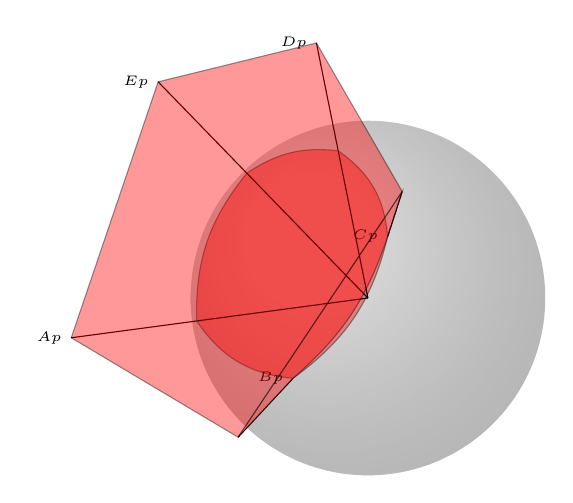
\begin{tikzpicture}[scale=1.3]
  \coordinate (O) at (0,0,0);
  \tdplotsetmaincoords{60}{165}
  \pgfmathsetmacro\R{sqrt(3)} 
  \fill[ball color=white!10, opacity=0.2, name path global=C] (O) 
      circle (\R); % 3D lighting effect
  \begin{scope}[tdplot_main_coords, shift={(0,0)}]
    \pgfmathsetmacro\R{sqrt(3)} 
    \pgfmathsetmacro{\thetavec}{0};
    \pgfmathsetmacro{\phivec}{0};
    \pgfmathsetmacro{\gammav}{0};
    \tdplotsetrotatedcoords{\phivec}{\thetavec}{\gammav};

    %%theta scales up and down Z, phi irotates hortizontally
    \def\thetaA{90}
    \def\phiA{0}
    \sphToCart{\R}{\thetaA}{\phiA}
    \coordinate (A) at (\x,\y,\z);

    \def\thetaA{90}
    \def\phiA{50}
    \sphToCart{\R}{\thetaA}{\phiA}
    \coordinate (B) at (\x,\y,\z);

    \def\thetaA{40}
    \def\phiA{85}
    \sphToCart{\R}{\thetaA}{\phiA}
    \coordinate (C) at (\x,\y,\z);
    
    \def\thetaA{10}
    \def\phiA{0}
    \sphToCart{\R}{\thetaA}{\phiA}
    \coordinate (D) at (\x,\y,\z);
    
    \def\thetaA{45}
    \def\phiA{-30}
    \sphToCart{\R}{\thetaA}{\phiA}
    \coordinate (E) at (\x,\y,\z);

    %%draw area
    \draw[fill=red, opacity=0.4] (A) to [bend right=25] (B) 
        to [bend right=20] (C) to [bend right=25]  (D) to [bend right = 20] (E) to [bend right=20] (A);
    
    %%Draw polygon
    \pgfmathsetmacro\R{3} 
    \def\thetaA{90}
    \def\phiA{0}
    \sphToCart{\R}{\thetaA}{\phiA}
    \coordinate (Ap) at (\x,\y,\z);

    \def\thetaA{90}
    \def\phiA{50}
    \sphToCart{\R}{\thetaA}{\phiA}
    \coordinate (Bp) at (\x,\y,\z);

    \def\thetaA{40}
    \def\phiA{85}
    \sphToCart{\R}{\thetaA}{\phiA}
    \coordinate (Cp) at (\x,\y,\z);
    
    \def\thetaA{10}
    \def\phiA{0}
    \sphToCart{\R}{\thetaA}{\phiA}
    \coordinate (Dp) at (\x,\y,\z);
    
    \def\thetaA{45}
    \def\phiA{-30}
    \sphToCart{\R}{\thetaA}{\phiA}
    \coordinate (Ep) at (\x,\y,\z);
    
    %%draw lines to sphere
    \foreach \x in {Ap,Dp,Ep} {
        \draw[color=black] (O)--(\x) node[anchor=east] {\tiny $\x$};
        }
    \foreach \x in {B,C} {
        \draw[color=black] (\x p)--(\x) node[anchor=east] {\tiny $\x p$};
        }
    %%draw polygon
    \draw[fill=red, opacity=0.4] (Ap) to (Bp) 
        to  (Cp) to [dashed]  (Dp) to (Ep) to(Ap);
    \draw[fill=red, opacity=0.4] (Bp) to (Cp) to (C) to [bend left = 15] (B);
    
    %% axis
    % \coordinate (XX) at (3,0,0) ;
    % \coordinate (YY) at (0,3,0) ;
    % \coordinate (ZZ) at (0,0,3) ;
    % \draw[-latex] (O) -- (XX) node[anchor=east] {$X$};
    % \draw[-latex] (O) -- (YY) node[anchor=north] {$Y$};
    % \draw[-latex] (O) -- (ZZ) node[anchor=south] {$Z$};
  \end{scope}
\end{tikzpicture}

\end{document}